\documentclass[a4paper]{article}
\usepackage[ngerman]{babel}
\usepackage[utf8]{inputenc}
\usepackage{multicol}
\usepackage{calc}
\usepackage{ifthen}
\usepackage[landscape]{geometry}
\usepackage{amsmath,amsthm,amsfonts,amssymb}
\usepackage{color,graphicx,overpic}
\usepackage{listings}
\usepackage[compact]{titlesec} %less space for headers
\usepackage{mdwlist} %less space for lists
\usepackage{pdflscape}
\usepackage{verbatim}
\usepackage[hidelinks,pdfencoding=auto]{hyperref}
\usepackage{fancyhdr}
\usepackage{lastpage}
\pagestyle{fancy}
\fancyhf{}
\fancyhead[L]{Rechnerarchitekturen 2}
\fancyfoot[L]{\thepage/\pageref{LastPage}}
\renewcommand{\headrulewidth}{0pt} %obere Trennlinie
\renewcommand{\footrulewidth}{0pt} %untere Trennlinie

\pdfinfo{
    /Title (Rechnerarchitekturen 2 - Cheatsheet)
    /Creator (TeX)
    /Producer (pdfTeX 1.40.0)
    /Author (Robert Jeutter)
    /Subject ()
}

% This sets page margins to .5 inch if using letter paper, and to 1cm
% if using A4 paper. (This probably isn't strictly necessary.)
% If using another size paper, use default 1cm margins.
\ifthenelse{\lengthtest { \paperwidth = 11in}}
    { \geometry{top=.5in,left=.5in,right=.5in,bottom=.5in} }
    {\ifthenelse{ \lengthtest{ \paperwidth = 297mm}}
    {\geometry{top=1.3cm,left=1cm,right=1cm,bottom=1.2cm} }
    {\geometry{top=1.3cm,left=1cm,right=1cm,bottom=1.2cm} }
    }
  
% Redefine section commands to use less space
\makeatletter
\renewcommand{\section}{\@startsection{section}{1}{0mm}%
                                {-1ex plus -.5ex minus -.2ex}%
                                {0.5ex plus .2ex}%x
                                {\normalfont\large\bfseries}}
\renewcommand{\subsection}{\@startsection{subsection}{2}{0mm}%
                                {-1explus -.5ex minus -.2ex}%
                                {0.5ex plus .2ex}%
                                {\normalfont\normalsize\bfseries}}
\renewcommand{\subsubsection}{\@startsection{subsubsection}{3}{0mm}%
                                {-1ex plus -.5ex minus -.2ex}%
                                {1ex plus .2ex}%
                                {\normalfont\small\bfseries}}
\makeatother

% Don't print section numbers
\setcounter{secnumdepth}{0}

\setlength{\parindent}{0pt}
\setlength{\parskip}{0pt plus 0.5ex}    
% compress space
\setlength\abovedisplayskip{0pt}
\setlength{\parskip}{0pt}
\setlength{\parsep}{0pt}
\setlength{\topskip}{0pt}
\setlength{\topsep}{0pt}
\setlength{\partopsep}{0pt}
\linespread{0.5}
\titlespacing{\section}{0pt}{*0}{*0}
\titlespacing{\subsection}{0pt}{*0}{*0}
\titlespacing{\subsubsection}{0pt}{*0}{*0}

\begin{document}

\begin{multicols}{2}
  \footnotesize
  \begin{description*}
    \item[Ausführungszeit] $t[s]=\frac{\text{Taktzyklen [Takte]}}{\text{Frequenz [Hz]}} =\frac{C}{f}$
    \item[Leistung absolut] $L_{abs}[MIPS]=\frac{\text{Befehlsanzahl}}{\text{Ausführungszeit [s]}*10^6}=\frac{n}{t*10^6}$
    \item[Leistung relativ] $L_{rel}[MIPS]=\frac{\text{Referenzzeit [s]}}{\text{Ausführungszeit [s]}}*\text{RefLeistung [MIPS]} = \frac{t_{ref}}{t_mess}*L_{ref}$
    \item[Clocks per Instruction] $CPI=\frac{\text{Taktzyklen [Takte]}}{\text{Befehlsanzahl}} =\frac{C}{n}$
    \item[Gewichtete mittlere] $CPI_{G}=\sum (CPI_{Bef.gr.}*\text{Rel.Häufigkeit}_{Bef.gr.})=\sum_{i=1}^n(CPI_i*p_i)$
    \item[Instructions per Clock] $IPC=\frac{Befehlsanzahl}{\text{Taktzyklen [Takt]}}=\frac{n}{C}$
    \item[Speedup] $S_n=\frac{1}{AnteilSeriell + Overhead + \frac{AnteilParallel}{AnzahlProzessoren}}=\frac{1}{ A_{seriell} + o(n) + \frac{ A_{parallel} }{ n }}$
    \item[Effizienz] $E_n=\frac{Speedup}{AnzahlProzessoren}=\frac{S_n}{n}$
  \end{description*}
\end{multicols}

\centering{
  \begin{tabular}{l | c | c | c | c | c}
    Bezeichnung  & Konflikterkennung & Issue-Struktur & Scheduling                & Hauptmerkmal                 & Beispiele                          \\\hline
    Superskalar  & Hardware          & Dynamisch      & Statisch                  & In-order Execution           & Sun UltraSPARC II/ III             \\
    Out of Order & Hardware          & Dynamisch      & Dynamisch mit Spekulation & Out of Order mit Spekulation & Pentium III, Pentium 4, MIPS 10000 \\ 
    VLIW         & Software          & Statisch       & Statisch                  & Keine Konflikte              & Trimedia, diverse DSPs
  \end{tabular}
}

\raggedright
\footnotesize
\begin{multicols}{3}
  
  % multicol parameters
  % These lengths are set only within the two main columns
  \setlength{\columnseprule}{0.25pt}
  \setlength{\premulticols}{1pt}
  \setlength{\postmulticols}{1pt}
  \setlength{\multicolsep}{1pt}
  \setlength{\columnsep}{2pt}
  
  
  \section{Prozessorarchitekturen}
  \paragraph{CISC} complex instruction set computer
  \begin{itemize*}
    \item Einfache und komplexe Befehle
    \item Heterogener Befehlssatz
    \item verschiedene Taktzahl pro Befehl
    \item Viele Befehlscode-Formate mit unterschiedlicher Länge
    \item Mikroprogrammwerk                             
    \item Vermischung von Verarbeitungs \& Speicherbefehlen
    \item schwierig, unter CPI = 2 zu kommen
  \end{itemize*}
  
  \paragraph{RISC} reduced instruction set computer
  \begin{itemize*}
    \item wenige, einfache Befehle
    \item orthogonaler Befehlssatz   
    \item meist 1 Takt pro Befehl
    \item wenige Befehlscode-Formate mit einheitlicher Länge 
    \item Direktverdrahtung
    \item Trennung von Verarbeitungs \& Speicherbefehlen  
    \item hohe Ausführungsgeschwindigkeit $(CPI \leq 1)$
  \end{itemize*}
  
  \paragraph{MIPS}
  \begin{itemize*}
    \item Microprocessor without interlocked pipeline stages
    \item 32-bit Architektur/64-bit Erweiterung
  \end{itemize*}
  
  \begin{center}
    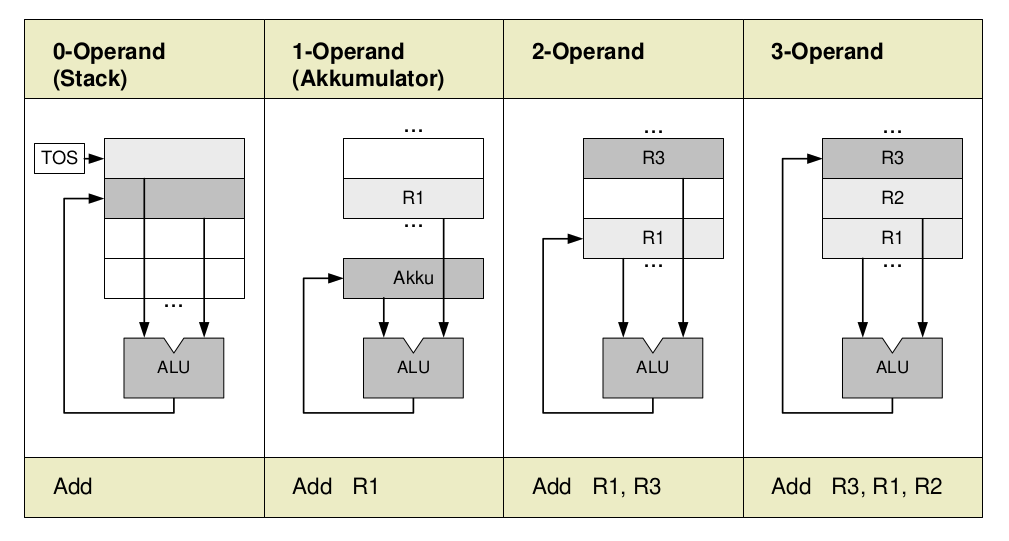
\includegraphics[width=\textwidth/7]{Assets/RA2_Operanden.png}
    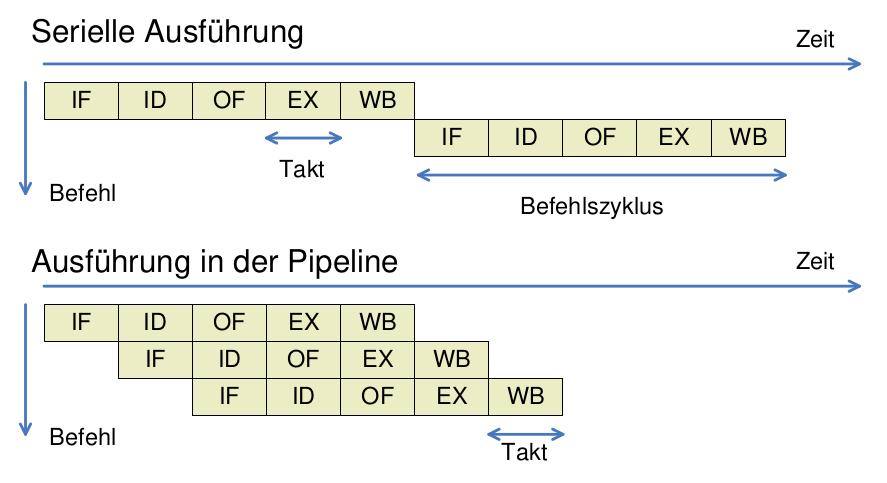
\includegraphics[width=\textwidth/7]{Assets/RA2_pipelineCPU.png}
    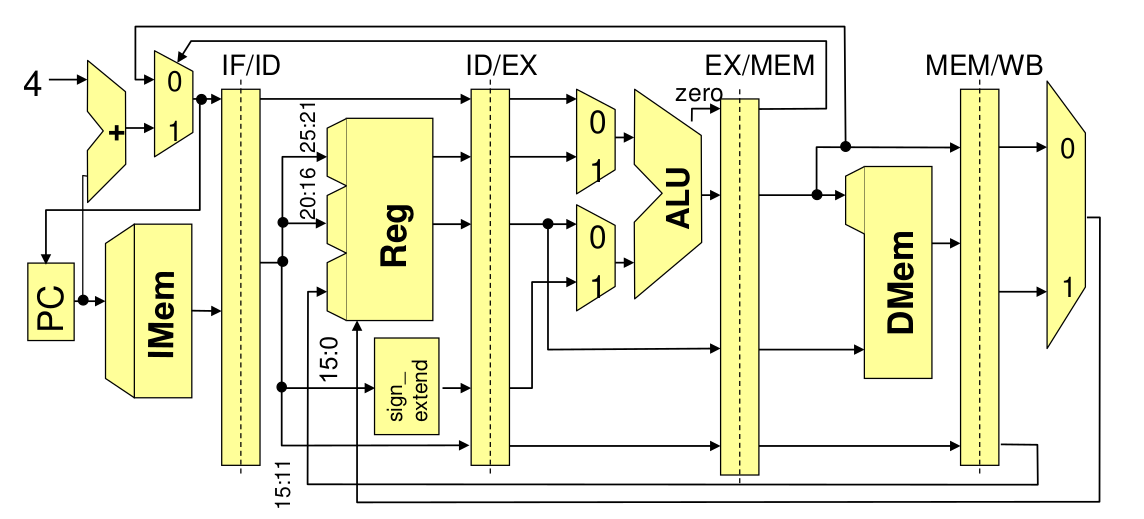
\includegraphics[width=\textwidth/4]{Assets/RA2_mehrzyklenCPU.png}
  \end{center}
  
  Aufgaben der einzelnen Phasen
  \begin{description*}
    \item[Befehlsholphase] Lesen des aktuellen Befehls; separater zur Vermeidung von Konflikten mit Datenzugriffen
    \item[Dekodier \& Register-Lese-Phase] Lesen der Register möglich wegen fester Plätze für Nr. im Befehlswort
    \item[Ausführungs \& Adressberechnungsphase] Berechnung arithmetischer Funktion o. Adresse für Speicherzugriff
    \item[Speicherzugriffsphase] Wird nur bei Lade \& Speicherbefehlen benötigt
    \item[Abspeicherungsphase] Speichern in Register, bei Speicherbefehlen nicht benötigt
  \end{description*}
  
  \paragraph*{Hazards}
  \begin{itemize*}
    \item resource hazards: Ressourcenabhängigkeiten
    \item data hazards: Datenabhängigkeiten
    \begin{description*}
      \item[Antidatenabhängig] WAR (write after read)
      \item[Ausgabeabhängig] WAW (write after write)
      \item[Datenabhängigkeit] RAW (read after write)
    \end{description*}
    \item control hazards: Kontrollabhängigkeiten
    \begin{itemize*}
      \item Gleichheit der Register in ID-Stufe prüfen
      \item Sprungziel in separatem Adressaddierer in ID berechnet
    \end{itemize*}
  \end{itemize*}
  
  \subsection{Sprungvorhersage}
  \paragraph{Einfache lokale Prädiktoren}
  \begin{itemize*}
    \item Vorhersage: bedingter Sprung genommen oder nicht
    \item Prädiktion anhand der Historie des betrachteten Sprungs
    \item Historie eines Sprungs wird mit 1 bis n Bits gepuffert
  \end{itemize*}
  
  \paragraph{Einfache Sprungvorhersage (1 Bit)}
  \begin{itemize*}
    \item Branch prediction buffer oder branch history table
    \item Kleiner Speicher, der mit (Teil der) Adresse des Sprungbefehls indiziert wird
    \item Verwendet nur wenige untere Bits der Adresse
    \item Enthält 1 Bit: Sprung beim letzten Mal ausgeführt (taken) oder nicht (not taken)
    \item Prädiktion: Sprung verhält sich wie beim letzten Mal
    \item Nachfolgebefehle ab vorhergesagter Adresse holen
    \item Falls Prädiktion fehlerhaft: Prädiktionsbit invertieren
    \item Sprünge, gleicher Adressen im Indexteil, werden selber Zelle im branch prediction buffer zugeordnet
    \item Einfachste Art von Puffer
    \item Hat eine bestimmte Kapazität
    \item Kann nicht für alle Sprünge Einträge enthalten
    \item Reduziert branch penalty, wenn branch delay $>$ Berechnung der Zieladresse mit branch p. buffer
    \item Prädiktion kann fehlerhaft sein
    \item Prädiktion kann von anderem Sprungbefehl stammen
  \end{itemize*}
  
  \paragraph{Einführung von Tag Bits}
  \begin{itemize*}
    \item Sprünge, gleicher Adressen im Indexteil, in selber Zelle
    \item Tag: gültiger Eintrag, falls Tag-Bits gleich sind
    \item Fehlerrate 1-Bit-P in Schleifenkonstrukten doppelt so hoch wie Anzahl ausgeführter Sprünge
  \end{itemize*}
  
  \paragraph{2 Bit Vorhersagen}
  \begin{itemize*}
    \item Änderung der Vorhersage nur, wenn 2 falsche Vorhersagen in Folge
    \item 2-Bit Branch-Prediction Buffer: Speicherung der Historie, Befehlsadressen als Zugriffsschlüssel
  \end{itemize*}
  % !{Sprungvorhersage; Quelle RA2 Vorlesung 2020/21](Assets/RA2_Sprungvorhersage.png)
  
  \paragraph{n-Bit Prädikator}
  \begin{itemize*}
    \item Verwendet n-Bit Zähler
    \item Sättigungsarithmetik (kein wrap around bei Überlauf)
    \item Kann Werte zwischen $0$ und $2^{n-1}$ annehmen
    \item Wenn Zähler größer als Hälfte des Maximums $(2^{n-1})$: Vorhersagen, dass Sprung ausgeführt wird
    \item Zähler bei ausgeführtem Sprung inkrementiert und bei nicht ausgeführtem dekrementiert
    \item Praxis: 2-Bit Prädiktor ähnlich gut wie n-Bit Prädiktor
  \end{itemize*}
  
  \paragraph{Korrelierende Prädikatoren}
  \begin{itemize*}
    \item Betrachtet nur Verhalten eines Sprungs; rein lokal
    \item Verbesserung durch Betrachtung anderer Sprünge
    \item erhält so korrelierenden/zweistufigen Prädiktor
    \item Prinzip: Aufgrund globaler Information wird einer von mehreren lokalen Prädiktoren ausgewählt
    \item Beziehen zur Vorhersage des Verhaltens Kontext-Information mit ein
    \item Prädiktor benutzt globale Kontext-Bits, um einen von mehreren lokalen Prädiktoren auszuwählen
    \item Betrachten wiederholte Ausführung des Codefragments
  \end{itemize*}
  
  \paragraph{Zweistufiger Prädiktor}
  \begin{itemize*}
    \item Es existieren 2 lokale Prädiktoren, beide je 1-Bit
    \item Kontext: Letzter Sprung wurde (nicht) ausgeführt
    \item Anhand des Kontexts wird lokaler Prädiktor für die Vorhersage des aktuell betrachteten Sprungs ausgewählt
    \item Letzter Sprung ist i.a. nicht gleich aktuellem Sprung
    \item Notation des Prädiktorstatus:$<X>/<Y>$ mit
    \item $<X>$: Vorhersage, falls letzter Sprung not taken
    \item $<Y>$: Vorhersage, falls letzter Sprung taken
    \item $<X>\vee<Y>$ Vorhersagen: entweder T oder NT
  \end{itemize*}
  
  \paragraph{(m,n)-Prädiktor}
  \begin{itemize*}
    \item Betrachtet das Verhalten der letzten m Sprünge, um aus $2^m$ vielen lokalen Prädiktoren einen n-Bit Prädiktor auszuwählen
    \item Höhere Vorhersagegenauigkeit
    \item Erfordert kaum Hardwareaufwand
    \item Sprunggeschichte in m-Bit Schieberegister gespeichert
    \item Vorhersagepuffer adressiert via Konkatenation von unteren Adressbits der Sprungbefehlsadresse
  \end{itemize*}
  
  \begin{center}
    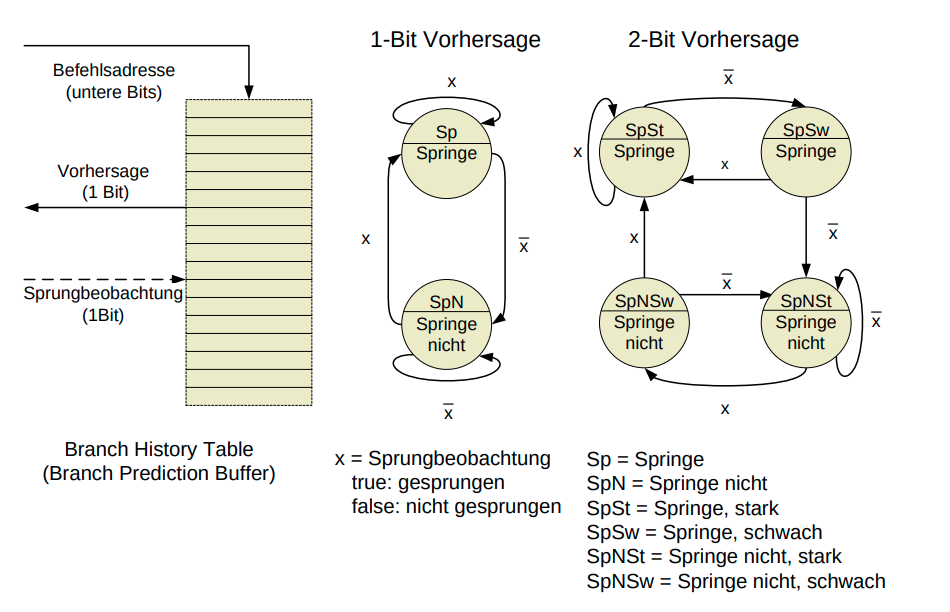
\includegraphics[width=\textwidth/7]{Assets/RA2_Vorhersagen.png}
  \end{center}
  
  \paragraph{High Performance Befehlsdekodierung}
  reine Vorhersage eines Sprungs i.d.R. nicht ausreichend
  \begin{itemize*}
    \item Befehlsstrom mit großer Bandbreite erforderlich
    \item Kontrollflussabhängigkeiten dürfen nicht wahrnehmbar sein 
    \item Pufferung von Sprungzielen und nicht nur Vorhersage des Sprungverhaltens (branch target buffer)
    \item Integrierte Einheit für das Holen der Befehle
    \item Vorhersage von Rücksprungadressen (bei Prozeduraufruf)
  \end{itemize*}
  
  \paragraph{Branch Target Buffer}
  5-stufige Pipeline, Auswertung von Sprungbedingungen in EX
  \begin{itemize*}
    \item Branch delay von 2 Takten
    \item mit Sprungvorhersage (branch prediction buffer)
    \item Zugriff erfolgt in ID (Adresse des Sprungbefehls in IF bekannt)
    \item Nächste vorhergesagte Instruktion kann erst nach ID geholt werden
    \item Branch delay = 1, falls Prädiktion korrekt
    \item Mit Pufferung des Sprungziels
    \item Zugriff auf branch target buffer erfolgt in IF
    \item Verhalten wie „echter“ Cache, adressiert mit Sprungbefehlsadresse
    \item Liefert vorhergesagte Adresse als Ergebnis
    \item Keine Verzögerung, falls Prädiktion korrekt
    \item Zusätzliche Speicherung auch des Sprungziels
    \item bei geschickter Organisation bleibt das Fließband immer gefüllt
    \item Sprünge kosten dann effektiv keine Zeit; $CPI <1$ mögl.
  \end{itemize*}
  Eigenschaften
  \begin{itemize*}
    \item Verzögerung durch Sprung vollständig vermieden, da bereits in IF Entscheidung über nächsten Befehlszähler getroffen
    \item Entscheidung allein auf Basis des PC getroffen wird, muss überprüft werden ob Adresse im Puffer
    \item Speicherung nur für Sprünge notwendig, die als ausgeführt vorhergesagt werden
    \item entsteht ursprüngliche Sprung-Verzögerung plus Aufwand zur Aktualisierung des Vorhersagepuffers
  \end{itemize*}
  
  \paragraph{Integrierte Befehls-Hol-Einheit (IF Unit)}
  Insbesondere mit Blick auf multiple-issue Prozessoren eigene (autonome) funktionale Einheit für Befehlsholphase
  \begin{itemize*}
    \item führt Befehlscodes in Pipeline ein
    \item Sprungvorhersage wird Teil der Befehlsholphase
    \item Instruction Pre-fetch: Insbes. um mehrere Befehle pro Takt liefern zu können, läuft Befehlsholen weiterer Dekodierung voraus
    \item Zugriff auf Befehlsspeicher: Bei mehreren Befehlen pro Takt mehrere Zugriffe erforderlich (bei Cache auf ggfs. mehrere cache lines). Werden hier koordiniert/geplant
    \item Befehlspuffer: Befehle können hier (lokal im Prozessor!) von Issue-Stufe nach Bedarf abgerufen werden
  \end{itemize*}
  
  \paragraph{Vorhersage von Rücksprungadressen}
  Vorhersage indirekter Sprünge (d.h. bzgl. Basisadresse in Register)
  \begin{itemize*}
    \item Hauptverwendung: Rückkehr aus Prozeduraufrufen
    \item MIPS: Prozeduraufruf per $jal$, Rückkehr per $jr$
    \item Vorhersage mit branch target buffer schlecht, da Aufruf aus unterschiedlichen Codeteilen heraus möglich
    \item Methode: (Stack-) Speicher für Rücksprungadressen
    \item Push bei Prozeduraufruf (call)
    \item Pop bei Rücksprung (return)
    \item Vorhersagequalität „perfekt“, wenn Stack-Puffer größer als maximale Aufruftiefe
  \end{itemize*}
  
  \section{Multiple-Issue-Architekturen}
  \paragraph{Mehrere Ausführungseinheiten}
  \begin{itemize*}
    \item Weitere Leistungssteigerung $CPI < 1$
    \item Mehrere Befehle pro Takt ausgeben
    \item Zwei Grundtypen von multiple-issue Prozessoren
    \begin{itemize*}
      \item Superskalar: var. Anzahl von Befehlen pro Takt
      \item VLIW/EPIC: Feste Anzahl von Befehlen ausgegeben, definiert durch Befehlscode (Planung der Issue-Phase durch Compiler)
    \end{itemize*}
  \end{itemize*}
  % !{In Order Pipeline; Quelle RA2 Vorlesung 2020/21](Assets/RA2_in-order-pipeline.png)
  
  \subsection{Superskalar}
  \begin{itemize*}
    \item IF holt 1-n Befehle von Instruction Fetch Unit
    \item Befehlsgruppe, die potentiell ausgegeben werden kann = issue packet
    \item Konflikte bzgl. Befehlen im issue packet werden in Issue-Stufe in Programmreihenfolge geprüft
    \item Befehl ggfs. nicht ausgegeben (und alle weiteren)
    \item Aufwand für Prüfung in Issue-Stufe groß!
    \item Wegen Ausgewogenheit der Pipeline-Stufen ggfs. Issue in mehrere Stufen unterteilen = nicht-trivial
    \item Parallele Ausgabe von Befehlen limitierender Faktor superskalarer Prozessoren
  \end{itemize*}
  
  \paragraph{MIPS mit statischem Scheduling}
  \begin{itemize*}
    \item Annahme: 2 Befehle pro Takt können ausgegeben werden (1x ALU, Load/Store plus 1x FP)
    \item Einfacher als 2 beliebige Befehle (wegen „Entflechtung“)
    \item 2 Befehlsworte holen (64-Bit Zugriff, komplexer als 1 B.)
    \item Prüfen, ob 0/1/2 Befehle ausgegeben werden können
    \item Befehle ausgeben an korrespondierende funk. Einheiten
    \item Prüfen auf Konflikte durch Entflechtung vereinfacht
    \item Integer und FP-Operationen nahezu unabhängig
    \item Abhängigkeiten nur bei Speichertransfers möglich (von Integer-ALU für FP ausgeführt)
    \item Leistungssteigerung nur bei geeignetem Anteil von FP-Operationen und Verflechtung durch Compiler
  \end{itemize*}
  
  \paragraph{Dynamisches Scheduling} in-order-execution
  \begin{itemize*}
    \item Jeder Befehl, der aus der Instruction fetch-Einheit kommt, durchläuft Scoreboard
    \item Wenn für Befehl alle Daten/Operanden bekannt sind und Ausführungseinheit frei ist, wird Befehl gestartet
    \item Alle Ausführungseinheiten melden abgeschlossene Berechnungen dem Scoreboard
    \item Scoreboard erteilt Befehlen die Berechtigung zum Abspeichern von Ergebnissen und prüft, ob dadurch neue Befehle ausführbereit werd
    \item Zentrale Datenstruktur: Scoreboard (für Befehlsstatus)
    \item load/store-Architektur
    \item mehrere funktionale Einheiten
    \item Scoreboarding für MIPS nur sinnvoll wenn:
    \item für FP-Pipeline (Operationen mit mehreren Taktzyklen)
    \item mehrere funktionale Einheiten (zB: 2xMult, Div, Add, Int)
  \end{itemize*}
  % !{Out Of Order Execution; Quelle RA2 Vorlesung 2020/21](Assets/RA2_out-of-order-execution.png)
  
  \paragraph{Verfahren von Tomasulo}
  \begin{itemize*}
    \item erlaubt bei Ausgabe-/Antidatenabhängigkeiten Reihenfolge zu vertauschen
    \item Umbenennung der Register
    \item verschiedenen Benutzungen eines Registers werden verschiedene Speicherzellen zugeordnet
    \item Jeder funktionalen Einheit wird eine Reservation Station zugeordnet
    \item Reservation Stations enthalten die auszuführende Operation und die Operanden/tags des Operanden
    \item Sind alle Operanden bekannt und ist die funktionale Einheit frei, so kann die Bearbeitung beginnen
    \item Am Ende der Bearbeitung wird das Ergebnis von allen Einheiten übernommen, die das Ergebnis benötigen
    \item Verteilen der Daten erfolgt vor der Abspeicherung im Registerspeicher
    \item Aus den tag bits geht hervor, aus welcher Einheit der Operand kommen muss
    \item Registeradressen werden dynamisch auf größere Anzahl von Plätzen in den Reservation Stations abgebildet
    \item Performance-Beschränkungen wegen weniger Register werden so umgangen
  \end{itemize*}
  
  \paragraph{Register Renaming}
  \begin{itemize*}
    \item Verwendung temporärer Register für (logisch) neue möglicherweise interferierende Belegung
    \item Alle Namenskonflikte durch Umbenennung auflösbar
    \item Wichtige Hardwarestruktur: Reservation Stations
    \item Zugeordnet zu funktionalen Einheiten (pro Einheit)
    \item Puffern Operanden für Befehle (sobald verfügbar)
    \item Müssen nicht aus Registern gelesen werden
    \item Ausstehende Operanden verweisen auf Reservation Station, die Eingabe bereitstellen
    \item Bei aufeinander folgenden Schreibzugriffen auf Register: Nur letzter für Aktualisierung des Inhalts verwendet
    \item Wichtige Eigenschaften der Verwendung von Reservation Stations anstelle des zentralen Registersatzes
    \item Konfliktdetektion und Ausführungskontrolle verteilt
    \item Informationen in Reservation Stations bei den funktionalen Einheiten bestimmen, wann Ausführung eines Befehls möglich ist
    \item Ergebnisse werden direkt zu den funktionalen Einheiten (in jeweiliger Reservation Station) weitergereicht
    \item Erweiterte Form des Forwarding
    \item Realisiert implizit Register Renaming durch gemeinsamen Ergebnisbus (common data bus)
  \end{itemize*}
  
  \subsection{Multiple-Issue mit dynamischem Scheduling}
  \begin{itemize*}
    \item Nachteil von statischem Scheduling: Latenzzeiten werden ca. mit Länge des issue packets skaliert
    \item Längere Verzögerung für Load/Stores bzw. Branches
    \item Lösung: Erweiterung des Tomasulo-Algorithmus auf Multiple-Issue
    \item Sequentielles Ausgeben mehrerer Befehle an Reservation Stations innerhalb eines Taktes
    \item oder „Verbreiterung“ der Ausgabe-Logik (issue logic) zur Behandlung mehrerer Operationen parallel
  \end{itemize*}
  
  \paragraph{VLIW} Very Long Instruction Word
  \begin{itemize*}
    \item Befehlszuordnung und Konfliktvermeidung durch Compiler
    \item Compiler muss Zeitbedarf der Speicherzugriffe in Befehlsplanung einbeziehen
    \item Befehlsstrom mit Tupel von Befehlen
    \item flexibel bei Reaktion auf Laufzeitereignisse
    \item VLIW hat festes Befehlsformat; höhere Codedichte
    \item Forwarding Hardware - nach EX können Daten vom nächsten Befehl genutzt werden
    \item WB erfolgt erst darauf
    \item Datenabhängigkeitsproblem wird verringert
    \item MUX nutzt eher Pufferdaten als Registerdaten
    \item verschiedene parallele Ausführungseinheiten
    \item Verteilung von Maschinencode direkt vom Befehlswort im Speicher vorgegeben
    \item für jede Ausführungseinheit dezidierte Anweisungen
    \item meist für stark parallelisierbare Aufgaben verwendet
    \item Vorteile:
    \begin{itemize*}
      \item parallele Architektur des Prozessors kann während der Programmerstellung zur Optimierung genutzt werden
      \item Keine aufwendige Prozessorhardware zur Befehlsverteilung erforderlich
      \item Ausführungszeiten sind im wesentlichen bekannt
    \end{itemize*}
    \item Nachteile:
    \begin{itemize*}
      \item Aufwendigere Compiler
      \item Schlechte Prozessorauslastung bei ungünstigem Code
      \item Rekompilierung für den Prozessor erforderlich
      \item Größerer Speicherbedarf, wenn Code nicht parallelisiert werden kann
    \end{itemize*}
  \end{itemize*}
  % !{VLIW Dynamisch; Quelle RA2 Vorlesung 2020/21](Assets/RA2_VLIW-dynamisch.png)
  
  \paragraph{EPIC} Explicitely Parallel Instruction Computing = IA64
  \begin{itemize*}
    \item im wesentlichen Prinzip des VLIW-Prozessors
    \item Umsortieren der Befehle und Auflösung der Abhängigkeiten wird durch Compiler durchgeführt
    \item Hauptnachteil: Neukompilierung erforderlich
    \item Keine statische Aufteilung auf Funktionseinheiten
    \item Effizienteres Befehlswort
    \item Keine Verwendung von zwangsweise NOPs
  \end{itemize*}
  verschiedene Ansätze, um die Prozessorlogik zu vereinfachen
  \begin{enumerate*}
    \item Bedingte Befehlsverarbeitung
    \begin{itemize*}
      \item Befehl abhängig von Statusbit ausgeführt
      \item Sprungvorhersage kann bei einfachen if-then-else Zweigen entfallen
      \item then/else Befehle parallel, nur einer ausgeführt
    \end{itemize*}
    \item Statische Sprungvorhersage (Compiler)
    \item Die Optimierung wird dem Compiler überlassen
    \item Spekulatives Laden von Operanden
    \begin{itemize*}
      \item Möglichst geringe Wartezeit auf Operanden
      \item Schon im Compiler werden entsprechende Ladebefehle vorgezogen
    \end{itemize*}
  \end{enumerate*}
  % !{VLIW Vergleich; Quelle RA2 Vorlesung 2020/21](Assets/RA2_VLIW-vergleich.png)
  
  \subsection{Simultaneous Multithreading (SMT)}
  % !{SMT; Quelle RA2 Vorlesung 2020/21](Assets/RA2_Simultaneous-Multithreading.png)
  \begin{itemize*}
    \item Modellprozessor I (2-fach Superskalar)
    \item Modellprozessor II (2-fach Out-of-Order)
  \end{itemize*}
  
  \subsection{Speicherhierarchie}
  \begin{itemize*}
    \item Große Speicher sind langsam
    \item Anwendung verhalten sich üblicherweise lokal
    \item Häufig benötigte Speicherinhalte in kleinen Speichern
  \end{itemize*}
  \begin{center}
    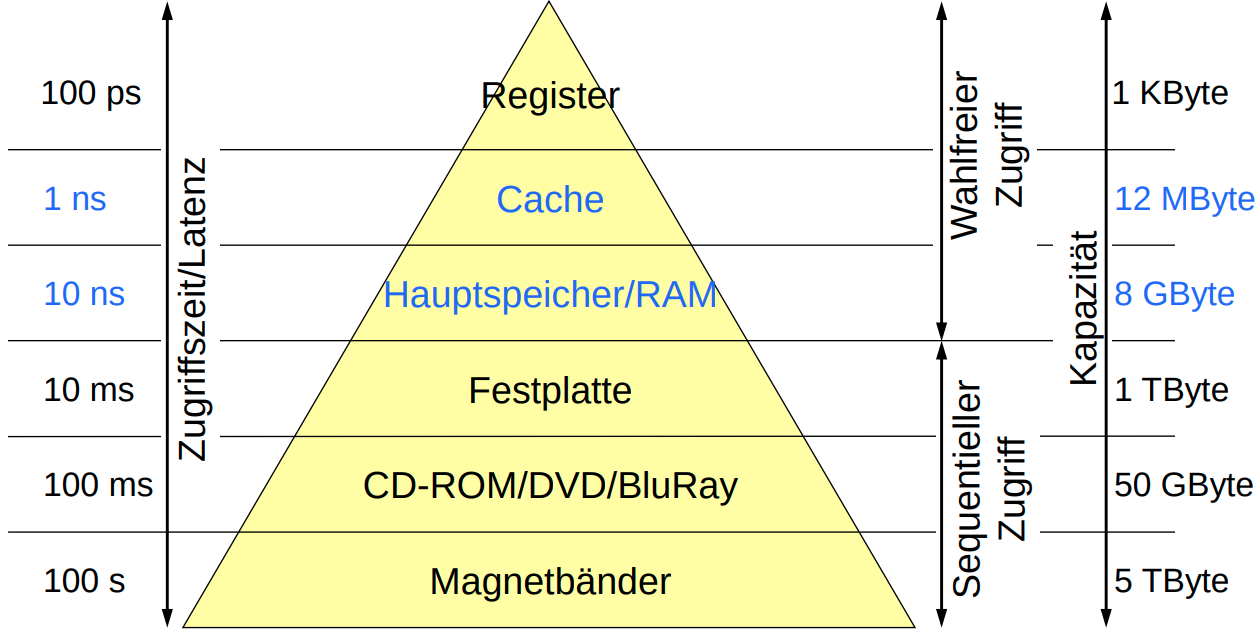
\includegraphics[width=\textwidth/4]{Assets/RA2_Speicherhierarchie.png}
  \end{center}
  
  \vfill
  \section{Speicherarchitekturen}
  \paragraph{Adresspipelining}
  \begin{itemize*}
    \item Aufteilen des Speicherzugriffs in mehrere Phasen
    \item parallele gestaffelte Abarbeitung dieser Phasen für mehrere Speicherzugriffe
    \item Adresse auslesen/dekodieren; Daten mit Prozessor
  \end{itemize*}
  % !{Pipelining; Quelle RA2 Vorlesung 2020/21](Assets/RA2_Adresspipelining.png)
  Lesezugriff auf Speicher
  \begin{itemize*}
    \item Matrixaufbau eines Speichers
    \item Aufteilen der Speicheradresse in Zeilen- und Spalten
    \item Dekodierung der Zeilenadresse bestimmt Select-Leitung
    \item Komplette Zeile wird in den Zeilenpuffer geschrieben
    \item Dekodierung der Spaltenadresse bestimmt Datenwort
  \end{itemize*}
  
  \subsection{Speicher Interlacing}
  \begin{itemize*}
    \item Speicheraufteilung in mehrere physische Bände
    \item Adressen nicht kontinuierlich in den Bänden, sondern wechseln von Band zu Band
    \item nahezu gleichzeitiges Benutzen der Daten möglich (Daten-/Adressbus verhindern Parallelität)
  \end{itemize*}
  
  \paragraph{Burst Mode} Blocktransfer
  \begin{itemize*}
    \item Auslesen des kompletten Zeilenpuffers durch automatisches Inkrementieren der Spaltenadresse
    \item Prozessor gibt eine Adresse, Speicher liefert n Datenworte (Adr, Adr+1,..., Adr+n-1)
    \item falls folgende Datenworte genutzt werden, war für n Datenworte nur 1 Speicherzugriff (Zeit) nötig
  \end{itemize*}
  
  \subsection{Typischer DRAM-Speicher}
  \begin{itemize*}
    \item Adressleitungen werden i.d.R. gemultiplext
    \item gleiche Adressleitungen werden einmal zur Auswahl der Zeile verwendet, dann zur Auswahl der Spalte
    \item Einsparung von Leitungen, gerade für große Speicher
    \item Steuerleitungen RAS/CAS codieren
    \item RAS (Row Address Strobe): Bei fallenden Flanke auf RAS ist anliegende Adresse Zeilenadresse
    \item CAS (Column Address Strobe): Bei fallenden Flanke auf CAS ist anliegende Adresse Spaltenadresse
    \item Zeilenadressdecoder liefert Select-Leitung für eine Zeile
    \item Komplette Zeile wird in einen Zwischenpuffer übernommen und zurückgeschrieben
    \item Nur 1 Transistor und 1 Kondensator pro Speicherzelle, statt 6 Transistoren bei SRAM
    \item Integrationsdichte Faktor 4 höher als bei SRAMs
    \item Weniger Platzbedarf aber Langsamerer Zugriff wegen Zwischenspeicherung und Auffrischung
    \item während Auffrischung kann nicht zugegriffen werden
    \item Hoher Energieverbrauch bei Aktivität/Inaktivität
    \item Ladungsverlust Ausgleich durch periodische Auffrischung
  \end{itemize*}
  %Interleaving
  % !{Interleaving; Quelle RA2 Vorlesung 2020/21](Assets/RA2_Interleaving.png)
  
  \subsection{Cache Speicher}
  \begin{itemize*}
    \item kleiner, schneller prozessornaher Speicher
    \item Puffer zwischen Hauptspeicher und Prozessor
    \item CPU weiß nicht dass Cache zwischengeschaltet ist
    \item es wird immer zuerst im Cache nachgeschaut (kostet Zeit)
    \item 90\% der Zeit verbringt ein Programm in 10\% des Codes
    \item Cache besteht aus Cache Tabelle
    \begin{description*}
      \item[voll assoziativ] Adressvergl. der kompletten Adresse
      \item[direct-mapped] Adressvergleich nur über Teiladresse
      \item[mehr-wege-assoziativ] mehrere Adressverg. parallel
    \end{description*}
    \item Schreibstategien
    \begin{description*}
      \item[Write Back] Cache sammelt Schreibvorgänge und aktualisiert Speicher nach Anweisung
      \item[Copy Back] Rückschreiben erfolgt erst, wenn Cache-Zeile bei Miss verdrängt wird
      \item[Write Through] Daten werden sowohl im Cache als auch im Hauptspeicher aktualisiert
      % !{Write Trough vs Write Back; Quelle RA2 Vorlesung 2020/21](Assets/RA2_cache-write-trough-vs-back.png)
    \end{description*}
    \item Speicherverwaltung mit memory management günstiger vor dem Cache
    \item cache hit: benötigte Daten im Cache vorhanden
    \item cache miss: Zugriff auf den (Haupt-) Speicher
    %\item Prinzip eines Cache (Hit) !{Cachehit; Quelle RA2 Vorlesung 2020/21](Assets/RA2_Cachehit.png)
    \item Such-Einheit im Cache: Cache-Zeile (cache line)
    \item Blockgröße ist Anzahl der Worte, die im Fall eines cache misses aus Speicher nachgeladen werden
    \item Verbindung Speicher $\leftrightarrow$ Cache ist so entworfen, dass Speicher durch zusätzliches Lesen nicht langsamer wird
    \item Methoden dazu:
    \begin{itemize*}
      \item Schnelles Lesen aufeinanderfolgender Speicherzellen (Burst Mode)
      \item Interleaving (mehrere Speicher ICs mit überlappenden Zugriffen)
      \item Fließbandzugriff auf den Speicher (SDRAM)
      \item Breite Speicher übertragen mehrere Worte parallel
    \end{itemize*}
    %\item 2-Wege Cache (Datensicht) !{2 Wege Cache; Quelle RA2 Vorlesung 2020/21](Assets/RA2_2-wege-cache.png)
    \item Ersetzungs-Strategien
    \begin{description*}
      \item[Zufall] zu ersetzende Block zufällig ausgewählt
      \item[FIFO] älteste Block ersetzt
      \item[LRU](least recently used) längsten nicht zugegriffen
      \item[LFU](least frequently used) am seltensten gelesene
      \item[CLOCK] Zeiger im Uhrzeigersinn zeigt Eintrag
    \end{description*}
    \item Trefferquote $T=\frac{N_{Cache Zugriffe}}{N_{Cache Hit}}$
  \end{itemize*}
  
  \section{Spezialrechner}
  \subsection{Einchiprechner}
  \begin{itemize*}
    \item geringer Stromverbrauch, Wärme
    \item relativ geringer Befehlsdurchsatz
    \item einfacher Befehlssatz
    \item komplexer Rechner auf einem Chip (Ram/Rom intern)
    \item an Problem angepasst
    \item so Leistungsfähig wie nötig
    \item Anwendung: einfache Steuer-/Regelungsaufgaben
  \end{itemize*}
  
  \subsection{Digital-Signal-Prozessoren}
  \begin{itemize*}
    \item hohe Leistung, u.a. sich wiederholende, numerisch intensive Aufgaben
    \item pro Befehlszyklus kann man ausführen
    \begin{itemize*}
      \item mehrere ALU Funktionen (+Shifter)
      \item eine/mehrere MAC-Operationen
      \item ein/mehrere Speicherzugriffe
      \item spezielle Unterstützung effiziente Schleifen
    \end{itemize*}
    \item Die Hardware enthält
    \begin{itemize*}
      \item Eine oder mehrere MAC-Einheiten
      \item On-Chip- und Off-Chip-Speicher mit mehreren Ports
      \item Mehrere On-Chip-Busse
      \item Adressgenerierungseinheit
      \item größerer ROM, RAM (mit Stack), Cache
      \item externes Interface für Speicher und E/A
      \item DMA-Coprozessor
      \item mehrere universelle parallele E/A-Ports
      \item AD-Wandler meist nicht on-chip
    \end{itemize*}
    \item DSP's benutzung häufig VLIW
    \item Anwendung: Signal-/Bildverarbeitung
  \end{itemize*}
  
  \subsection{Pipeline Prozessoren}
  \begin{itemize*}
    \item Aufteilung eines Befehls in Teilbefehle
    \item parallele Abarbeitung verschiedener Teilbefehle
    \item Problem: bedingte Sprünge (unvorhergesehen)
    \begin{itemize*}
      \item LSG: Pipeline um 2 Schritte verzögern
      \item LSG: Sprungzielspekulation
    \end{itemize*}
    \item Problem: Datenabhängigkeit
    \begin{itemize*}
      \item LSG: Pipeline um 2 Schritte verzögern
      \item LSG: Out-of-Order Prinzip nutzen
      \item LSG: Forwarding Hardware
    \end{itemize*}
    \item Superpipelining - noch mehr Befehlsaufteilung
  \end{itemize*}
  
  \subsection{Skalare Prozessoren}
  \begin{itemize*}
    \item Mikroarchitektur
    \item Befehlszuordnung und Konfliktvermeidung geschieht durch Hardware
    \item Speicherzugriffe automatisch von Load/Store Einheit
    \item Befehlsstrom mit einfachem Befehl an EX-Einheit
    \item bessere Reaktion auf Laufzeitereignisse
    \item Spekulation möglich
    \item Superskalar ($\geq 2$ EX Einheiten)
    \begin{itemize*}
      \item Befehle in Befehlsfenster gespeichert
      \item Zuordnungseinheit wählt Befehl aus, die parallel verarbeitet werden können
    \end{itemize*}
  \end{itemize*}
  
  \paragraph{Multiprozessorarchitekturen}
  nach Flynn
  \begin{center}
    \begin{tabular}{ c | c | c}
                       & Ein Datenstrom & mehrere Datenströme \\\hline
      ein Befehlsstrom & SISD           & SIMD                \\
      mehrere Bs       & MISD           & MIMD 
    \end{tabular}
  \end{center}
  \begin{center}
    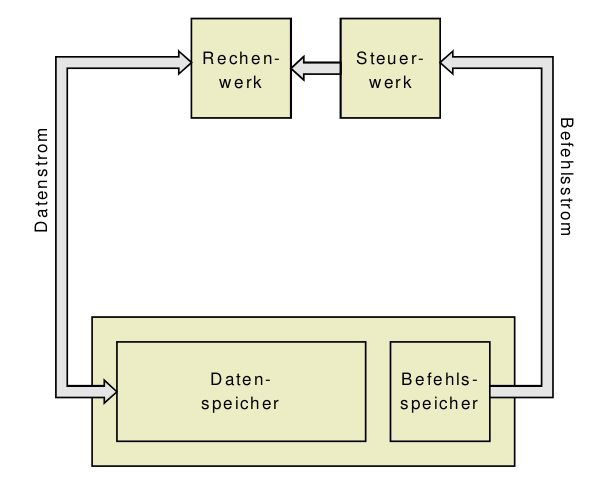
\includegraphics[width=\textwidth/13]{Assets/RA2_SISD.png}
    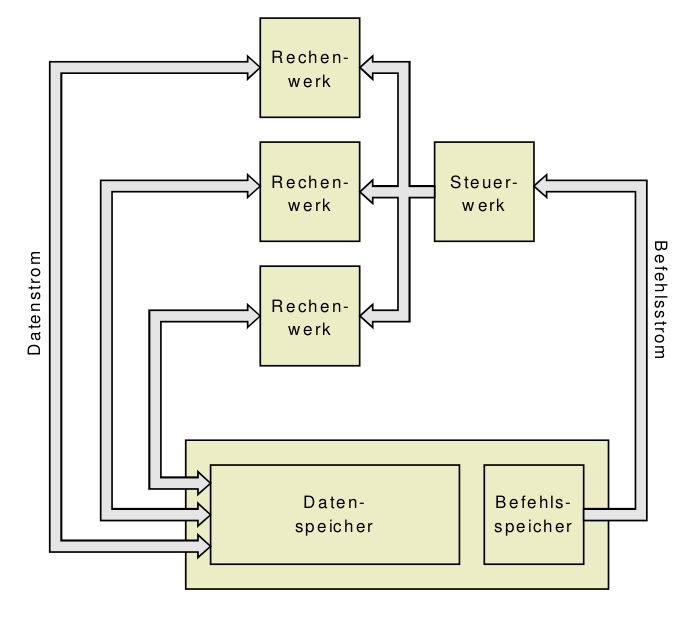
\includegraphics[width=\textwidth/13]{Assets/RA2_SIMD.png}
    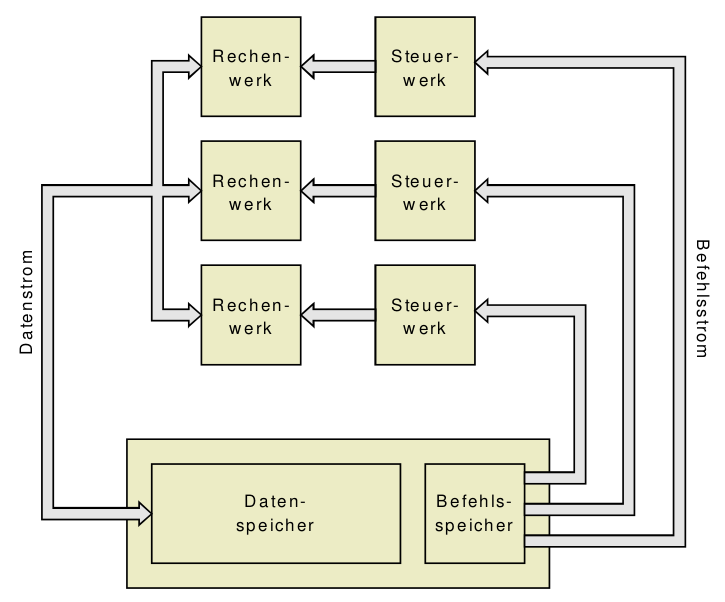
\includegraphics[width=\textwidth/13]{Assets/RA2_MISD.png}
    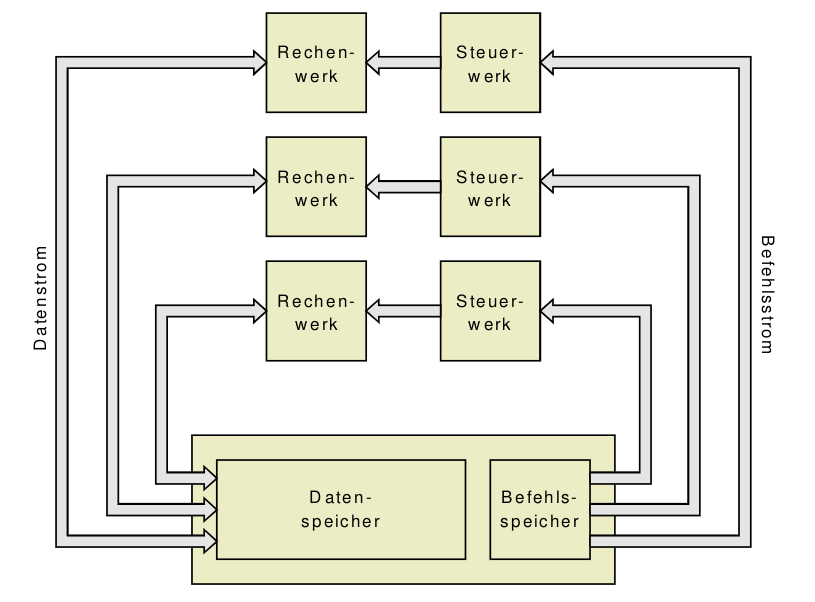
\includegraphics[width=\textwidth/13]{Assets/RA2_MIMD.png}
  \end{center}
  
  %Verbindungsnetzwerke
  % !{Verbindungsnetzwerke; Quelle RA2 Vorlesung 2020/21](Assets/RA2_Verbindungsnetzwerke.png)
  % !{Verbindungsnetzwerke2; Quelle RA2 Vorlesung 2020/21](Assets/RA2_Verbindungsnetzwerke2.png)
  
  %Dual-Core-System mit mehrstufiger Bushierarchie
  % !{Dual Core System; Quelle RA2 Vorlesung 2020/21](Assets/RA2_DualCoreSystem.png)
  
  %Reales Shared Memory System
  % !{Shared Memory System; Quelle RA2 Vorlesung 2020/21](Assets/RA2_SharedMemorySystem.png)
  
  \subsection{Kopplung}
  \begin{description*}
    \item[enge Kopplung] (shared memory)
    \begin{itemize*}
      \item parallelzugriff in Datenbreite des Prozessors
      \item schneller Datenaustausch 
      \item neu lokal benachbarte Rechner
      \item aus Sicht des Prozessors gemeinsamer Speicher
      \item Arbites - Zuteiler für Busanforderungen
    \end{itemize*}
    \item[lose Kopplung] (distributed memory)
    \begin{itemize*}
      \item meist seriell 1 bit breit
      \item langsamer da über Kommunikations-schnittstelle
      \item auch global verteilte Rechner
      \item verschiedene Speicher dem Prozessor bewusst
    \end{itemize*}
    \item[Kopplung] verändern
    \begin{itemize*}
      \item Wartezeit auf Speicher
      \item Kommunikationsaufwand
      \item Kommunikationsfähigkeit
    \end{itemize*}
  \end{description*}
  \begin{center}
    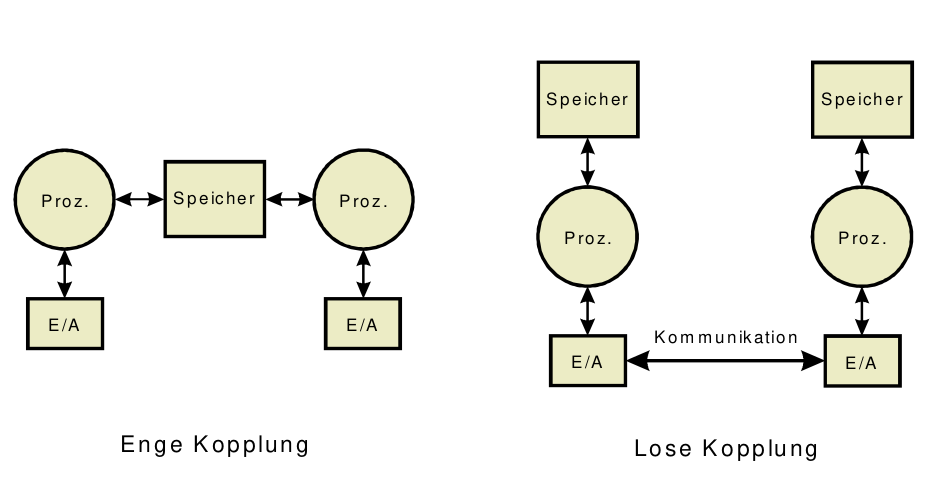
\includegraphics[width=\textwidth/7]{Assets/RA2_Enge und lose Kopplung.png}
    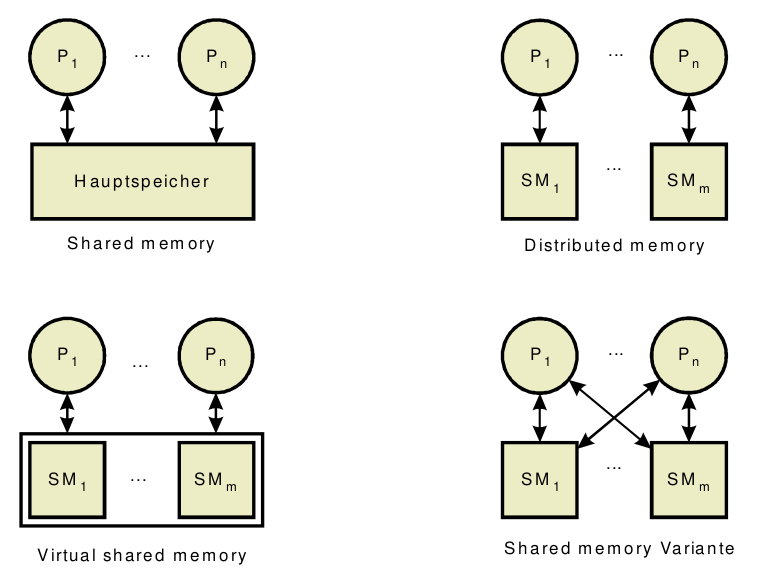
\includegraphics[width=\textwidth/7]{Assets/RA2_Speicherstrukturen.png}
  \end{center}
  
  \paragraph{Verbindungsnetzwerke}
  \begin{description*}
    \item[Linie] $KL_{max}=n-1$
    \item[Ring] $KL_{max}=\frac{n}{2}$
    \item[Torus 2D] $KL_{max}=\sqrt{n}-1$
    \item[Torus 3D] $KL_{max}=\frac{3}{2}\sqrt[3]{n}-1$
    \item[Hypercube] $iD=i$
    \item[Gitter] $iD=i*\sqrt[i]{n}-1$
  \end{description*}
  
  \subsection{Out-of-Order Architektur}
  \begin{itemize*}
    \item statt Pipeline bei Datenabhängigen Befehlen um 2 Schritte verzögern, datenunabhängige Befehle einschieben
    \item möglichst ständige Auslastung aller EX Einheiten
  \end{itemize*}
  
  \paragraph{Cache(daten)-Kohärenz}
  \begin{itemize*}
    \item Kohärenz: welcher Wert wird beim Lesen abgeliefert
    \item Bezug auf Lesen und Schreiben ein- und derselben Speicherzelle
    \item Definition: Ein Speichersystem heißt kohärent, wenn
    \begin{itemize*}
      \item geschriebene Werte werden wieder gelesen
      \item Schreibvorgänge derselben Zelle serialisiert
    \end{itemize*}
    \item Lösung des I/O-Problems: Zuordnung einer I/O-Einheit zu jedem Prozessor
    % !{Cache I/O Einheit; Quelle RA2 Vorlesung 2020/21](Assets/RA2_CacheIOEinheit.png)
    \item Hardware-Lösung: Aufwändig, schlechte Lokalität der Daten
    \item Gemeinsamer Cache für alle Prozessoren: Hoher Hardware-Aufwand, geringe Effizienz
    \item Unterscheidung in cacheable/non-cacheable Daten: Hoher Aufwand
  \end{itemize*}
  
  \paragraph{Snooping-Protokolle}
  \begin{itemize*}
    \item Caches aller Prozessoren beobachten alle Daten- übertragungen von jedem Cache zum Hauptspeicher
    \item Voraussetzung: broadcastfähiges Verbindungsnetzwerk
  \end{itemize*}
  \begin{description*}
    \item[Write Invalidate] Verändern eines Blocks im Speicher führt zur Invalidierung aller Cache-Kopien mit der gleichen Adresse
    \item[Write Update/Broadcast] Verändern eines Blocks im Speicher führt zur Modifikation aller anderen Cache-Blöcke mit der gleichen Adresse
  \end{description*}
  
  \paragraph{Copy-Back}
  \begin{itemize*}
    \item Copy-Back Caches führen zur temp. Inkonsistenz
    \item Lösung: exklusives Eigentumskonzept durch Zustandsgraph pro Cache-Block
    \item MESI (Modified, Exclusive, Shared, Invalid)
    \item Mischung zwischen Write-Through und Copy-Back
  \end{itemize*}

  \paragraph{MESI}
  \begin{center}
    \includegraphics[width=\textwidth/6]{Assets/RA2_MESI-Zustände.png}
    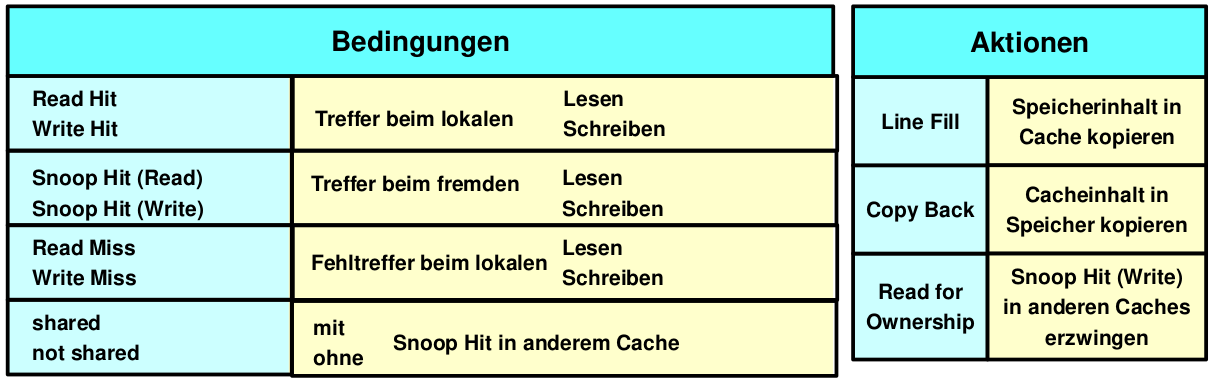
\includegraphics[width=\textwidth/6]{Assets/RA2_MESI-Bedingungen.png}
  \end{center}
  %\begin{description*}
  %  \item[Modified] Cache-Block wurde lokal geändert, die Kopie im Hauptspeicher ist ungültig. Will ein anderer Prozessor im Hauptspeicher lesen, so muss der Cache-Block erst in den Hauptspeicher zurückgeschrieben werden
  %  \item[Exclusive] (unmodified): Dieser Cache ist der einzige, der den Cache-Block enthält, Wert im Hauptspeicher ist gültig. Liest ein anderer Prozessor im Hauptspeicher, so muss die Zeile als shared markiert werden. Wird das Datum im Hauptspeicher verändert, ist der Cache-Block auf invalid zu setzen
  %  \item[Shared] (unmodified): Mehrere Caches enthalten Daten. Da alle bisher nur gelesen haben, sind Daten im Hauptspeicher gültig. Schreibzugriffe auf einen shared Cache-Block müssen immer zu einer Bus-Operation führen, damit die Cache-Blocks der anderen Caches auf invalid gesetzt werden können
  %  \item[Invalid] Cache-Block ist nicht geladen bzw. veraltet/ungültig
  %\end{description*}
  
  \paragraph{Bus-Operationen}
  \begin{description*}
    \item[Bus Read] Prozessor liest Wert eines Speicherblocks
    \item[Bus Read Exclusive] Prozessor überschreibt Wert eines Speicherblocks
    \item[Flush] Prozessor $P_i$ hat Speicherblock alleinig in seinem Cache, ein anderer Prozessor $P_j$ aber lesend oder schreibend auf diesen Block zugreift
  \end{description*}
  
  \paragraph{Steuersignale}
  \begin{itemize*}
    \item Invalidate-Signal: Invalidieren des Blocks in den Caches anderer Prozessoren
    \item Shared-Signal: Signalisierung, ob ein zu ladendes Datum bereits als Kopie im Cache vorhanden ist
    \item Retry-Signal: Aufforderung von Prozessor $P_i$ an Prozessor $P_j$, das Laden eines Datums vom Hauptspeicher abzubrechen, da der Hauptspeicher noch ein altes, ungültiges Datum besitzt und vorher aktualisiert werden muss. Das Laden durch $P_j$ kann danach wiederholt werden.
  \end{itemize*}
  
  Bewertung von Snooping-Protokollen
  \begin{itemize*}
    \item Leichte Implementierbarkeit bei Bus-basierten Shared Memory Systemen
    \item Snooping skaliert bei Bussen jedoch nicht
    \item Bei vielen beteiligten Prozessoren sinkt die effektive Bandbreite des Busses, da überproportional viele Invalidierungsnachrichten per Broadcast über den Bus gehen
    \item Punkt-zu-Punkt Netzwerke sind skalierbar, jedoch ist die Implementierung von Broadcasts hier aufwändig
    \item Für Snooping-Protokolle daher oft ungeeignet
  \end{itemize*}
  
  \paragraph{Directory-Protokolle}
  \begin{itemize*}
    \item Nur wenige Prozessoren teilen sich die gleichen Daten in vielen Anwendungen
    \item Directory-Protokolle nutzen Lokalitätsinformationen, um die Anzahl an Invalidierungsnachrichten zu minimieren
    \item Nachrichten gehen nur an Prozessoren, die eine Kopie des Cache-Blocks besitzen
    \item Directory-Protokolle skalieren daher auch für Netze ohne Broadcast-Fähigkeit
    \item Presence Flag Vector: Im Hauptspeicher abgelegter Bit-Vektor für jeden einzelnen Speicherblock (1 Bit pro Prozessor/Cache + Statusbits (dirty, modified))
    \item Problem: Wachstum des Speicherbedarfs linear mit Anzahl der Prozessoren
  \end{itemize*}
  
\end{multicols}
\end{document}